\documentclass[a4paper]{ltxdoc}
\usepackage{lmodern}			% Usa a fonte Latin Modern			
\usepackage[T1]{fontenc}		% seleção de códigos de fonte.
\usepackage[utf8]{inputenc}		% determina a codificação utiizada (conversão automática dos acentos)
\usepackage{hyperref}  			% controla a formação do índice
\usepackage{parskip}			% espaçamento entre os parágrafos
\usepackage{microtype} 			% para melhorias de justificação
\usepackage{morefloats}			% permite mais floats
\usepackage[absolute]{textpos}
\usepackage{tabularx}
\usepackage[table]{xcolor}
\usepackage{graphicx}
% Babel e ajustes
\usepackage[english,brazil]{babel}		% idiomas
\addto\captionsbrazil{
    %% ajusta nomes padroes do babel
    \renewcommand{\bibname}{Refer\^encias}
    \renewcommand{\indexname}{\'Indice}
    \renewcommand{\listfigurename}{Lista de ilustra\c{c}\~{o}es}
    \renewcommand{\listtablename}{Lista de tabelas}
    %% ajusta nomes usados com a macro \autoref
    \renewcommand{\pageautorefname}{p\'agina}
    \renewcommand{\sectionautorefname}{se{\c c}\~ao}
    \renewcommand{\subsectionautorefname}{subse{\c c}\~ao}
    \renewcommand{\paragraphautorefname}{par\'agrafo}
    \renewcommand{\subsubsectionautorefname}{subse{\c c}\~ao}
    \renewcommand{\paragraphautorefname}{subse{\c c}\~ao}
}  

\usepackage{color}
\definecolor{thered}{rgb}{0.65,0.04,0.07}
\definecolor{thegreen}{rgb}{0.06,0.44,0.08}
\definecolor{thegrey}{gray}{0.5}
\definecolor{theshade}{rgb}{1,1,0.97}
\definecolor{theframe}{gray}{0.6}
\definecolor{blue}{RGB}{41,5,195}
% \newcommand{\orientador}{Prof. Dr. Calebe de Paula Bianchini}
\newcommand{\orientador}{Prof. Dr. Pedro Paulo Balbi de Oliveira}
\newcommand\tab[1][1cm]{\hspace*{#1}}
\IfFileExists{listings.sty}{
  \usepackage{listings}
\lstset{%
	language=[LaTeX]TeX,
	columns=flexible,
	basicstyle=\ttfamily\small,
	backgroundcolor=\color{theshade},
	frame=single,
	tabsize=2,
	rulecolor=\color{theframe},
	title=\lstname,
	escapeinside={\%*}{*)},
	breaklines=true,
	commentstyle=\color{thegrey},
	keywords=[0]{\fichacatalografica,\errata,\folhadeaprovacao,\dedicatoria,\agradecimentos,\epigrafe,\resumo,\siglas,\simbolos,\citacao,\alineas,\subalineas,\incisos},
	keywordstyle=[0]\color{thered},
	keywords=[1]{},
	keywordstyle=[1]\color{thegreen},
	breakatwhitespace=true,
	alsoother={0123456789_},
	inputencoding=utf8,
	extendedchars=true,
	literate={á}{{\'a}}1 {ã}{{\~a}}1 {é}{{\'e}}1 {è}{{\`{e}}}1 {ê}{{\^{e}}}1 {ë}{{\¨{e}}}1 {É}{{\'{E}}}1 {Ê}{{\^{E}}}1 {û}{{\^{u}}}1 {ú}{{\'{u}}}1 {â}{{\^{a}}}1 {à}{{\`{a}}}1 {á}{{\'{a}}}1 {ã}{{\~{a}}}1 {Á}{{\'{A}}}1 {Â}{{\^{A}}}1 {Ã}{{\~{A}}}1 {ç}{{\c{c}}}1 {Ç}{{\c{C}}}1 {õ}{{\~{o}}}1 {ó}{{\'{o}}}1 {ô}{{\^{o}}}1 {Õ}{{\~{O}}}1 {Ó}{{\'{O}}}1 {Ô}{{\^{O}}}1 {î}{{\^{i}}}1 {Î}{{\^{I}}}1 {í}{{\'{i}}}1 {Í}{{\~{Í}}}1,
}
\let\verbatim\relax
 	\lstnewenvironment{verbatim}[1][]{\lstset{##1}}{}
}

\usepackage[alf]{abntex2cite}	% citacoes


% COMANDOS PROPRIOS
% \newcommand{\abnTeX}{}
% \newcommand{\abnTeXForum}{}
\newcommand{\abnTeXSite}{}

\title{\protect\parbox{\textwidth}{\protect\centering \textbf{Conservabilidade de estados de autômatos celulares elementares com atualizações assíncronas por prioridade da vizinhança}}}

%   \thanks{Este documento
%   se referete ao \textsf{abntex2} versão \fileversion,
%   de \filedate.}
  

\author{Marcelo Vironda Rozanti\\\abnTeXSite Felipe Stefanelli de Aguiar Silva\\\abnTeXSite} 

\date{\today}

\hypersetup{
  pdftitle={Conservabilidade de estados de autômatos celulares elementares com atualizações assíncronas por prioridade da vizinhança},
  pdfauthor={Marcelo Vironda Rozanti}{Felipe Stefanelli de Aguiar Silva},
  pdfkeywords={Asynchronous priority-based updating Elementary Cellular Automata, New Kind of Science, Discrete dynamical systems, Number-conserving}, 
  pdfproducer={Marcelo Vironda Rozanti},
  pdfcreator={vim+LaTeX+abnTeX2},
  colorlinks=true,
  linkcolor=black,
  citecolor=black,
  urlcolor=blue
}

% \EnableCrossrefs
\CodelineIndex
% \RecordChanges
\hyphenpenalty=1000

\begin{document}

\thispagestyle{empty}
\huge{\centerline{UNIVERSIDADE PRESBITERIANA MACKENZIE}}

\bigskip
\bigskip

\centerline{\large{FACULDADE DE COMPUTAÇÃO E INFORMÁTICA}}

\makeatletter
\vfill
\large{\centering{\@author}}

\vspace*{\fill}

\large{Conservabilidade de estados de autômatos celulares elementares com}
\large{\centerline{atualizações assíncronas por prioridade da vizinhança}}

\vspace*{\fill}
\large{\centerline{SÃO PAULO}}
\large{\centerline{2019}}

\pagebreak

\large{\centering{\@author}}
\vfill
\large{\centerline{\@title}}
\vfill
\vspace*{\fill}

Orientador: \orientador
\\
\\
\\


\large{\centerline{SÃO PAULO}}
\large{\centerline{2019}}

\begin{textblock}{6}(9,9)
% Projeto do Trabalho de Conclusão de Curso apresentado à Faculdade de Computação e Informática da Universidade Presbiteriana, desenvolvida como requisito parcial para aprovação na disciplina de Metodologia da Pesquisa em Computação, ministrada pelo professor Dr. Everton Knihs, do curso de Ciência da Computação.
\end{textblock}

\maketitle

\begin{abstract}
Autômatos Celulares são sistemas computacionais discretos e abstratos que se têm provado úteis como modelos genéricos de complexidade e representação de diversas dinâmicas em uma varidade de áreas científicas. Estes sistemas podem ser especificados puramente em termos matemáticos e até implementados em estruturas físicas. Muitos deles podem computar funções e resolver problemas algorítmicos. O presente projeto explora um conjunto fundamental deles, chamados Automatos Celulares Elementares com um tipo específico de atualização assíncrona baseada em prioridade com a esperança de encontrar modelos conservativos que podem ser usados em uma variedade de aplicações práticas. O código correspondende a este trabalho pode ser acessado no repositório \url{https://github.com/mvrozanti/TCC}.
\end{abstract}
Palavras-chave: Autômatos celulares elementares com atualização assíncrona por prioridade, New Kind of Science, Sistemas dinâmicos discretos, Conservabilidade

\vfill

\selectlanguage{english}
\begin{abstract}
Cellular Automata are discrete, abstract computational systems that have proved useful as general models of complexity and representations of dynamics on a variety of scientific fields. These systems can be specified in purely mathematical terms and be implemented in physical structures. Many of them can compute functions and solve algorithmic problems. The present project attempts to explore a fundamental subset of them, called Elementary Cellular Automata with a specific kind of prioriy-based asynchronous updating in the search of number-conserving models, which can be used for a variety of practical applications. The implementation developed is hosted at \url{https://github.com/mvrozanti/TCC}.
\end{abstract}
Keywords: \@pdfkeywords

\break

\selectlanguage{brazil}
\renewcommand{\contentsname}{\centerline{\Large Sumário}}

\tableofcontents

\listoftables

\listoffigures

\break

\section{INTRODUÇÃO}

\tab Este projeto teve como objetivo explorar propriedades conservativas em autômatos celulares elementares com atualização assíncrona baseada em prioridade da vizinhança.

% \tab Este projeto teve como objetivo otimizar algoritmos de \citeonline{overeinder1993application} cálculo de distância em arquiteturas com suporte a instruções dos conjuntos MMX (\textit{Multimedia Extensions}), SSE  (\textit{Streaming SIMD Extensions}) e AVX (\textit{Advanced Vector Extensions}) para a arquitetura de processadores com registradores de 512-bit de largura. Ao utilizar funções nativas do processador alvo, é possível atingir graus maiores de eficiência para uma determinada arquitetura. No entanto, segundo \citeonline{fast-sorting}: ``From one CPU generation to the next, improvements and changes are made at various levels. Some modifications are hidden from the programmer and might improve existing codes without any update. This includes the low-level modules (speculation, out-of-order execution, etc.) but also the CPU’s clock frequency. On the other hand, some new features and improvements require to be explicitly used''. O que é possível interpretar deste trecho é que determinadas modificações não necessitam de atualização no código. No entanto, outras melhorias devem ser necessariamente explicitadas para atingir ganhos mensuráveis.

\tab No caso do uso de supercomputadores, essa explicitação é essencial, tal como esclarece \cite[Abstract]{code-opt-simd}: ``One frequent concern about retargetable compilers, though, is their lack of machine-specific code optimization techniques in order to achieve highest code quality. While this problem is partially inherent to the retargetable compilation approach, it can be circumvented by designing flexible, configurable code optimization techniques that apply to a certain range of target architectures.''

% `` Um grande número de processadores têm extensões em aplicações multimídia'' \cite[p. 11]{multiplatform-simd-programming}.

\subsection{CONTEXTUALIZAÇÃO E RELEVÂNCIA}
% \tab O âmbito deste trabalho foi o uso de instruções SIMD: múltiplos operandos operados em paralelo em um único item de memória, como notado por \citeonline[p. 359]{stallings}.
% Compiladores atuais não otimizam todos os trechos críticos com o mesmo desempenho que a codificação direta composta por instruções explícitas. No caso de operações vetorizadas, é necessário dar ``dicas'' ou \textit{hints} ao compilador escolhido para garantir que certas otimizações sejam realizadas, como nos ensinam \citeonline[p. 192]{jeffers}: ``Even the most brilliantly conceived compiler cannot auto-vectorize many important loops without hints''.

\break

\subsection{OBJETO DE PESQUISA}
% \tab O objeto da pesquisa foi implementações e arquiteturas SIMD, com o suporte da documentação de funções intrínsecas x86 da Intel®, encontradas nos \textit{headers} \texttt{immintrin.h} para instruções AVX e \texttt{xmmintrin.h} para instruções SSE.

% \tab Como é visto em \citeonline[p. 8]{intel-avx-intro}, parte da etimologia das funções a serem empregadas é definida como a seguir:

\begin{table}[htb]
    \caption{Sufixos}
    \centerline{
        \begin{tabular}{|l|l|}
            \hline
            \textbf{Marcadores} & \textbf{Significado} \\
            \hline
            \texttt{[a/d]} & Ponto flutuante de precisão única ou dupla \\
            \hline
            \texttt{[i/u]nnn} & Inteiro com ou sem sinal de tamanho binário nnn onde nnn é 128, 64, 32, 16, ou 8  \\
            \hline
            \texttt{[ps/pd/sd]} & Valor único empacotado, valor duplo empacotado ou escalar duplo \\
            \hline
            \texttt{epi32} & Inteiro assinalado empacotado de 32-bit\\
            \hline
            \texttt{si256} & Inteiro 256-bit escalar\\
            \hline
        \end{tabular}
    }
\end{table}

\tab Esta tabela representa parte da lógica empregada na nomenclatura das funções, com o intuito de facilitar a compreensão da implementação e providenciar uma fácil iniciação ao usuário/programador.

\subsubsection{PROBLEMA DE PESQUISA} \label{problema}
\tab Muitos algoritmos de classificação, no que é pertinente ao campo de Machine Learning, se utilizam de medidas de similaridade tanto para o ``treino'' destes classificadores, como para o seu uso em produção. Estes algoritmos, por sua vez, requerem alto custo computacional. Pode-se criar uma solução mais eficiente que as atuais em arquiteturas paralelas de 512-bit? Ainda, como adaptar a solução a arquiteturas com maior largura de registradores? 

\break

\subsubsection{FÓRMULAS UTILIZADAS} \label{formulas}

\tab Por similaridade, entende-se a distância entre dois pontos em um espaço \textit{n-dimensional}, isto é, vetores de tamanho \textit{n}. As fórmulas a seguir denotam as medidas de distância utilizadas neste trabalho onde \textit{p} e \textit{q} são os pontos cuja distância se quer descobrir:

\tab Distância de Manhattan
\[d_{1}(\mathbf{p},\mathbf{q})=\sum_{i=1}^{n}\mid p_{i}-q_{i}\mid\]

\tab Distância Euclidiana
\[d_{2}(\mathbf{p},\mathbf{q})=\sqrt{\sum_{i=1}^{n}(q_{i}-p_{i})^{2}}\]

\tab Distância Cosseno
\[\alpha(\mathbf{p},\mathbf{q})={\frac{\sum\limits_{i=1}^{n}{p_{i}q_{i}}}{{\sqrt{\sum\limits _{i=1}^{n}{p_{i}^{2}}}}{\sqrt{\sum\limits_{i=1}^{n}{q_{i}^{2}}}}}}\]

% \break

\tab Visualização:

\begin{figure}[!htbp]
\centerline{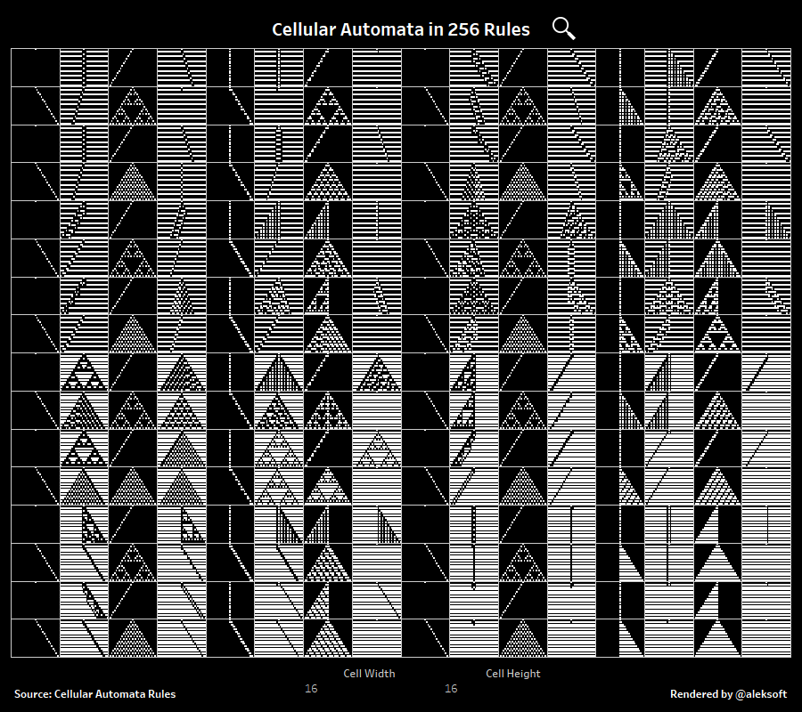
\includegraphics[width=\linewidth]{imgs/Picture1.png}}
\caption{Ilustração das 256 regras elementares}
\end{figure}

\tab Estas operações são usadas constante e intensivamente em algoritmos pertinentes ao domínio de Machine Learning como explicitado por \citeonline{wang2012distance} que ressaltam, ainda, o problema da Maldição da Dimensionalidade, também conhecido pelo anglicismo \textit{Curse of Dimensionality}, sendo possível depreender a importância da eficiência da implementação dos cálculos mencionados.

\subsubsection{HIPÓTESE BÁSICA} 
\tab É possível tirar vantagem da arquitetura de todo processador para resolver um determinado problema computacional, como visto por \citeonline{exploit-every-cycle} e \citeonline{exploiting-modern-hardware}. Testes de performance podem ser criados para verificar a superação de eficiência dos algoritmos em discussão.

\subsubsection{VARIÁVEIS}

\begin{itemize}
	\item Arquitetura alvo:\\
        \tab No contexto desta pesquisa, as implementações foram testadas no processador Xeon Platinum™ com suporte à instruções AVX-512, mas poderiam ser aplicadas em arquiteturas com maior largura de registradores.
	\item Compilador:\\
        \tab Os compiladores utilizados foram \texttt{icc/icpc} (Intel®) e \texttt{gcc/g++} (GNU), em diferentes momentos da pesquisa.
	\item Entrada ou pontos no espaço:\\
        \tab Pontos mencionados no item \ref{formulas} a serem escolhidos como argumento às funções.
\end{itemize}

\subsection{OBJETIVOS DO ESTUDO} 

\tab O objetivo desse estudo é ganhar maior compreensão sobre as capacidades e limitações encontradas no design eficiente de implementações em arquiteturas paralelas, bem como ampliar o conhecimento sobre compiladores e tradução código-máquina.

\subsubsection{OBJETIVO GERAL}
\tab Tornar algoritmos-base de cálculo de distância mais eficientes em determinadas arquiteturas.
\subsubsection{OBJETIVOS ESPECÍFICOS}

\tab Para alcançar o objetivo geral proposto para a resolução do problema de pesquisa, 
os seguintes objetivos específicos foram estabelecidos:

\begin{itemize}
    \item Identificação das  teorias  envolvidas  no  estudo  de  otimização  os aspectos que privilegiam o processo de desenvolvimento das otimizações. 
    \item Estudo no âmbito computacional atual dos processos de técnicas e boas práticas de otimização. 
    \item Identificação dos aspectos que qualificam alta-performance que devem ser observados na criação e desenvolvimento destes algoritmos. 
\end{itemize}

\subsection{JUSTIFICATIVA}

\tab Como já mencionado no item \ref{problema}, os algoritmos de classificação podem usar intensamente o cálculo de distância como instrumento intermediário e têm um impacto direto em sua performance. Qualquer ganho de eficiência nestes algoritmos de cálculo de distância em função da arquitetura pode ter uma influência notável na performance geral  dos classificadores em fase de treinamento ou em fase prática, ou, de produção, como afirmam \citeonline{effective-simd-vectorization} e \citeonline{optimization-pattern-recognition}.

\subsection{DELIMITAÇÃO DO ESTUDO} \label{delimitacao}
\tab Deve-se restringir a implementação dos algoritmos evidenciados no item \ref{problema}, para a arquitetura 512-bit:

\begin{itemize}
    \item Delimitação Organizacional: família Intel® de processadores
    \item Delimitação por Indicadores de Desempenho: testes com o intuito de verificar a eficiência do código proposto.
\end{itemize}

% \break

\subsection{ORGANIZAÇÃO DO ESTUDO}

Descrição dos capítulos:

\begin{enumerate}
    \item Introdução
        \subitem Preâmbulo deste trabalho.
    \item Referencial Teórico
        \subitem Sustentação argumentativa sobre o tema proposto.
    \item Metodologia de Pesquisa
        \subitem Sistematização dos instrumentos e processos de estudo empregados no presente trabalho.
    \item Cronograma
        \subitem Planejamento das tarefas necessárias para a conclusão deste trabalho, bem como suas expectativas de início e conclusão.
    \item Descrição da plataforma-alvo.
        \subitem Breve narrativa sobre ambiente e ferramentas utilizadas ao longo do estudo.
    \item Implementações de cálculo de distância.
        \subitem Detalhamento da solução final.
\end{enumerate}
 
\section{REFERENCIAL TEÓRICO}
\tab Em relação ao referencial teórico estudado neste TCC, foi de suma importância entender os seguintes tópicos:

\subsection{Computação SIMD} \label{comp-simd}
\tab O bloco fundamental dos conjuntos de instruções SIMD é composto por operadores booleanos, por exemplo, \texttt{AND}, \texttt{OR}, \texttt{XOR} e suas variantes, bem como deslocamentos lógicos e aritméticos, conversão de tipos e operações de seleção de dados como \texttt{max} e \texttt{min}, diz \citeonline[p. 29]{hughes2015single}.

\tab Extensões de CPU são, muitas vezes, específicas a uma família de processadores e podem ou não existir em mais de um compilador apenas, como é o caso de extensões SIMD, como dizem \citeonline{franchetti2005efficient}: "The most common language extension supplying such primitives is to provide within the C programming language function-call like intrinsic (or built-in) functions and new data types to mirror the instructions and vector registers. For most SIMD extensions, at least one compiler featuring these language extensions exists". 

\tab Isso significa que pode-se usar uma API para acessar estas funções instrínsecas ao processador nativo. A API, por sua vez, é composta por \textit{Programming Language Abstractions}, ainda segundo \citeonline[p. 15]{franchetti2005efficient}: "Recognizing the tedious and difficult nature of assembly coding, most hardware vendors which have introduced multi-media extensions have developed programming-language abstractions. These give an application developer access to the newly introduced hardware without having to actually write assembly language code. Typically, this approach results in a function-call-like abstraction that represents one-to-one mapping between a function call and a multi-media instruction. There are several benefits of this approach".

\subsection{Organização e arquitetura de computadores} \label{org-comp}
\tab Arquitetura computacional é um componente chave no desenvolvimento e o programador deve ter um entendimento prático sobre o tópico. ``It is concerned with all aspects of the design and organization of the central processing unit and the integration of the CPU into de computer system itself.'' \cite{stallings}. Isso mostra a importância da compreensão base de sistemas computacionais para aproveitar o equipamento ao máximo, visando aumento de performance e, consequentemente, uso eficiente de recursos, sejam estes financeiros ou temporais, como em qualquer outro projeto de software de qualidade.

\section{METODOLOGIA DA PESQUISA}
\tab No que tange à Metodologia empregada neste TCC, o trabalho teve início com uma revisão da literatura específica sobre o tema da pesquisa. Esta pesquisa abrange conceitos fundamentais de computadores de forma genérica (\ref{org-comp}) e específica (\ref{comp-simd}), bem como o ``estado da arte'' em termos de técnicas de otimizacão paralela e \textit{benchmarking} correspondente.

\subsection{ETAPAS DA PESQUISA}
\tab Para definir as etapas da pesquisa, foi necessário atender às delimitações de estudo (item \ref{delimitacao}), desenvolvendo, para cada tipo de distância especificado no item \ref{formulas}, suas respectivas implementações para AVX-512 com as APIs NVIDIA® OpenACC e Intel® Intrinsics. Excluindo funções intermediárias, isto é, que funcionam como instrumento interno, soma-se 6 funções implementadas, como descrito no Cronograma apresentado no item \ref{cron}.

\break

Assim, pode-se dizer que as etapas desenvolvidas neste estudo foram:

\begin{enumerate}
    \item Estudo da Documentação;
    \item Implementação da Distância Manhattan em Intel Intrinsics;
    \item Implementação da Distância Euclidiana em Intel Intrinsics;
    \item Implementação da Distância Cosseno em Intel Intrinsics;
    \item Implementação da Distância Manhattan em OpenACC;
    \item Implementação da Distância Euclidiana em OpenACC;
    \item Implementação da Distância Cosseno em OpenACC;
    \item Análise e testes das implementações;
    \item Artigo.
\end{enumerate}

\subsubsection{CONCEITOS EMPREGADOS}
\begin{itemize}
	\item Compilador:
        \subitem Programa capaz de traduzir instruções de uma linguagem de programação para outra.
	\item Entrada:
        \subitem Pontos num espaço \textit{n-dimensional}.
	\item Throughput:
        \subitem Número médio de tarefas completadas em uma determinada unidade temporal \cite[p. 299]{stallings}.
    \item Dados empacotados \cite[p. 379]{stallings}:
        \subitem Packed byte: oito bytes empacotados em uma quantidade 64-bit.
        \subitem Packed word: quatro palavras de 16-bit empacotadas em 64 bits.
        \subitem Packed doubleword: duas palavras duplas de 32-bit empacotadas em 64 bits.
    \item Extensões de CPU, melhor descritas no item \ref{comp-simd}
        \subitem MMX:
            Multimedia Extensions.
        \subitem SSE:
            Streaming SIMD Extensions.
        \subitem AVX:
            Advanced Vector Extensions.
    \item API:
        \subitem Application Programming Interface. 
\end{itemize}

\subsection{CLASSIFICAÇÃO DA PESQUISA}
\tab O tempo total previsto para a conclusão desta pesquisa é de 1 ano, como mostrado no capítulo \ref{cron}.

\subsubsection{NATUREZA DA PESQUISA}
\tab Esta é uma pesquisa Aplicada, já que sua aplicação prática é imediata.

\subsubsection{ABORDAGEM} 
\tab Esta pesquisa é baseada em cálculos, medidas objetivas e dados verificáveis.

\subsubsection{FINS} 
\tab Esta pesquisa foi voltada para encontrar caminhos, formas, maneiras e procedimentos para atingir um determinado fim, buscando definir um processo ou uma ferramenta que leve à solução do problema proposto (\ref{problema}).

\subsubsection{PESQUISA PROPOSITIVA} 
\tab Código-fonte, bem como suas instruções de compilação e documentação interna e externa utilizada para gerar o binário que ultrapasse soluções atuais para cálculo de distância nas arquiteturas alvo.

\subsubsection{MEIOS} 
\tab Quanto aos meios, foram utilizados os recursos mencionados na Bibliografia e Dados documentais (item \ref{documental}). Testes automatizados servirão para medir \textit{speedup} em relação a outros algoritmos conhecidos. 

\subsubsection{PESQUISA BIBLIOGRÁFICA}
\tab Para o andamento desta pesquisa foi necessário compreender a taxonomia de Flynn e programação paralela discorrida por \citeonline{stallings}, \citeonline{patterson}.

\subsubsection{PESQUISA DOCUMENTAL} \label{documental}
\tab Documentação de funções da família de instruções x86 Intel® Intrinsics extraído de \citeonline{intel-intrinsics-guide} e da API OpenACC da \citeonline{openacc-api}.

% \vfill
\break
\section{CRONOGRAMA} \label{cron}

\tab As atividades desta pesquisa se desenvolveram de acordo com o cronograma apresentado a seguir, no prazo de 12 meses:

\begin{table}[h]
    \caption{Cronograma de atividades}
    \centerline{
        \begin{tabular}{|l|l|l|l|l|l|l|l|l|l|l|l|l|}
          \hline
          ATIVIDADE & \multicolumn{12}{|c|}{MÊS} \\
          \hline
          &  1& 2& 3& 4& 5& 6& 7& 8& 9& 10& 11& 12 \\
          \hline
          Estudo da Documentação & \cellcolor{yellow} & \cellcolor{yellow} & & & & & &\cellcolor{yellow} & & & & \\
          \hline
          Implementação da Distância de Manhattan (Intel® Intrinsics) & & \cellcolor{yellow}& \cellcolor{yellow}& & & & & & & & & \\
          \hline
          Implementação da Distância de Euclidiana (Intel® Intrinsics) & & \cellcolor{yellow}& \cellcolor{yellow}& & & & & & & & & \\
          \hline
          Implementação da Distância de Cosseno (Intel® Intrinsics) & & & & \cellcolor{yellow}& \cellcolor{yellow}& & & & & & & \\
          \hline
          Implementação da Distância de Manhattan (OpenACC) & & & & \cellcolor{yellow}& \cellcolor{yellow}& & & & & & & \\
          \hline
          Implementação da Distância de Euclidiana (OpenACC) & & & & & & \cellcolor{yellow}& \cellcolor{yellow}& & & & & \\
          \hline
          Implementação da Distância de Cosseno (OpenACC) & & & & & & \cellcolor{yellow}& \cellcolor{yellow}& \cellcolor{yellow}& \cellcolor{yellow}& \cellcolor{yellow}& & \\
          \hline
          Artigo & & & & & & & & \cellcolor{yellow}& \cellcolor{yellow}& \cellcolor{yellow}& \cellcolor{yellow}& \cellcolor{yellow}\\
          \hline
    \end{tabular}
  }
\end{table}

% \break

\addcontentsline{toc}{section}{Referências}
\bibliography{cellz} \label{bib}

\end{document}
